% !TEX root = saveliev_physics_general_course_2.tex
%!TEX TS-program = pdflatex
%!TEX encoding = UTF-8 Unicode


\chapter[TỪ TRƯỜNG TRONG VẬT CHẤT]{TỪ TRƯỜNG\\ TRONG VẬT CHẤT}\label{chap:7}
\chaptermark{TỪ TRƯỜNG TRONG VẬT CHẤT}

\section{Sự Từ hóa của Vật liệu từ}\label{sec:7_1}

Ở các chương trước, chúng ta đã giả thiết là các vật dẫn mang dòng điện đều được đặt trong chân không.
Nếu các vật dẫn trên được đặt trong vật chất, từ trường sẽ thay đổi.
Lý do là vì mọi vật chất đều là vật liệu từ, \ie, đều có thể xuất hiện lưỡng cực từ dưới tác dụng của từ trường (bị từ hóa).
Vật chất bị từ hóa sẽ sinh ra từ trường $\vec{B}'$ mà sẽ chồng chập với từ trường $\vec{B}_0$ sinh ra bởi dòng điện.
Hai từ trường trên sẽ cho ra từ trường tổng là
\begin{equation}\label{eq:7_1}
    \vec{B} = \vec{B}_0 + \vec{B}'
\end{equation}

\noindent
[xem lại \eqn{2_8}].

Từ trường thực (vi mô) ở trong một vật liệu từ biến thiên mạnh khi ta di chuyển giữa các phân tử.
Do vậy, $\vec{B}$ sẽ được hiểu là từ trường trung bình (vĩ mô) (xem lại \sect{2_3}).
Để giải thích hiện tượng từ hóa, Ampere đã giả sử rằng có các dòng điện vòng chạy quanh các phân tử tạo thành vật chất (dòng điện vi mô).
Các dòng điện vòng trên đều có moment từ và đều sinh ra từ trường trong không gian quanh nó.
Khi không có từ trường ngoài, các dòng điện vi mô trên sẽ sắp xếp một cách hỗn loạn, do vậy mà từ trường tổng do chúng sinh ra sẽ bằng không.
Tương tự, moment từ của vật trên sẽ bằng không do các moment từ của từng phân tử trong nó định hướng một cách hỗn loạn.
Dưới ảnh hưởng của từ trường ngoài, moment lưỡng cực từ của các phân tử sẽ ưu tiên hướng theo một phương, làm cho vật bị từ hóa -- tổng moment từ của nó giờ khác không. Từ trường của các dòng điện vòng đơn lẻ trong trường hợp này cũng không triệt tiêu nhau nữa, do đó vật sẽ sinh ra từ trường $\vec{B}'$.

Sự từ hóa của vật chất có thể được đặc trưng bởi moment từ của một đơn vị thể tích vật chất từ.
Đại lượng này được gọi là \textbf{độ từ hóa} và được kí hiệu bởi $\vec{M}$.
Nếu chất trên được từ hóa không đồng đều, độ từ hóa tại một điểm sẽ được tính bởi biểu thức sau:
\begin{equation}\label{eq:7_2}
    \vec{M} = \frac{1}{\Delta{V}} \sum_{\Delta{V}} \ab{\vec{p}}{m}\,,
\end{equation}

\noindent
trong đó $\Delta{V}$ là một thể tích nhỏ vô cùng (từ góc nhìn vật lý) bao quanh điểm được xét, còn $\ab{\vec{p}}{m}$ là moment lưỡng cực từ của một phân tử.
Ta lấy tổng này trên mọi phân tử được chứa trong vùng có thể tích $\Delta{V}$ [giống với \eqn{2_4}].

Từ trường $\vec{B}'$, giống như từ trường $\vec{B}_0$, không có nguồn.
Do vậy, divergence của từ trường tổng trong \eqn{7_1} bằng không:
\begin{equation}\label{eq:7_3}
    \divop{\vec{B}} = \divop{\vec{B}_0} + \divop{\vec{B}'} = 0.
\end{equation}

\noindent
Do vậy, \eqn{6_96} và \eqn{6_95} không chỉ đúng cho từ trường trong chân không mà còn đúng cho từ trường trong vật chất nữa.

\section{Cường độ Từ trường}\label{sec:7_2}

Chúng ta hãy viết biểu thức cho curl của từ trường tổng \eqref{eq:7_1}:
\begin{equation*}
    \curlop{\vec{B}} = \curlop{\vec{B}_0} + \curlop{\vec{B}'}.
\end{equation*}

\noindent
Theo \eqn{6_103}, $\curlop{\vec{B}_0}=\mu_0\vec{j}$, trong đó $\vec{j}$ là mật độ dòng điện của dòng vĩ mô.
Tương tự, curl của vector $\vec{B}'$ sẽ phải tỉ lệ thuận với mật độ của dòng vi mô:
\begin{equation*}
    \curlop{\vec{B}'} = \mu_0 \ab{\vec{j}}{mol}.
\end{equation*}

\noindent
Do vậy, curl của từ trường tổng sẽ được tính bởi biểu thức sau
\begin{equation}\label{eq:7_4}
    \curlop{\vec{B}} = \mu_0 \parenthesis{\vec{j} + \ab{\vec{j}}{mol}}.
\end{equation}

Xem xét \eqn{7_4}, ta thấy rằng khi tính curl của từ trường trong vật chất từ, ta gặp phải vấn đề tương tự với điện trường trong điện môi [xem lại \eqn{2_16}]: để tính curl của $\vec{B}$, ta phải biết cả mật độ dòng điện của dòng vi mô và vĩ mô.
Tuy nhiên, mật độ dòng vi mô lại phụ thuộc vào giá trị của vector $\vec{B}$.
Cách xử lý vấn đề này cũng giống cách ta dùng trong \sect{2_5}: Ta sẽ tìm một đại lượng mà curl chỉ phụ thuộc vào mật độ dòng vĩ mô.

Để tìm dạng của đại lượng thứ cấp trên, chúng ta phải tìm phương trình miêu tả mật độ dòng vi mô $\ab{\vec{j}}{mol}$ theo độ từ hóa $\vec{M}$ (trong \sect{2_5} chúng ta đã biểu diễn mật độ của điện tích hưởng ứng theo độ phân cực của điện môi $\vec{P}$).
Để làm điều này, ta sẽ tính tổng đại số của các dòng điện vi mô được bao bởi vòng kín $\Gamma$. Tổng trên bằng
\begin{equation}\label{eq:7_5}
    \int_S \ab{\vec{j}}{mol} \ccdot \derivec{S},
\end{equation}

\noindent
trong đó  $S$ là diện tích của mặt được bao bởi vòng kín này.

Tổng đại số của các dòng vi mô chỉ bao gồm các dòng được ``xâu'' vào vòng kín (xem dòng $\ab{I}{mol}'$ trong \fig{7_1}).
Các dòng điện không được ``xâu'' vào vòng sẽ không cắt mặt được bao bởi vòng hoặc sẽ cắt nó hai lần theo hai chiều ngược nhau (xem dòng $\ab{I}{mol}''$ trong \fig{7_1}).
Hệ quả là các dòng trên sẽ không đóng góp vào tổng đại số của các dòng điện được bao bởi vòng kín.

\begin{figure}[!htb]
	\begin{minipage}[t]{0.48\linewidth}
		\begin{center}
			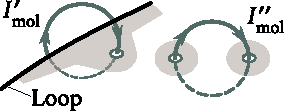
\includegraphics[scale=1]{figures/ch_07/fig_7_1.pdf}
			\caption[]{}
			\label{fig:7_1}
		\end{center}
	\end{minipage}
	\hfill{ }%space{-0.05cm}
	\begin{minipage}[t]{0.48\linewidth}
		\begin{center}
			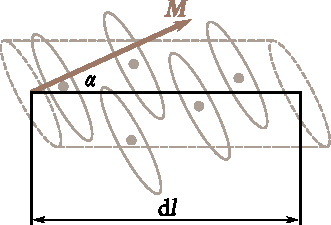
\includegraphics[scale=1]{figures/ch_07/fig_7_2.pdf}
			\caption[]{}
			\label{fig:7_2}
		\end{center}
	\end{minipage}
\vspace{-0.4cm}
\end{figure}

Nhìn vào \fig{7_2}, ta thấy rằng phần tử vòng kín $\deriv{l}$ mà tạo góc $\alpha$ với hướng của độ từ hóa $\vec{M}$ sẽ xâu qua các dòng điện vi mô có tâm nằm trong hình trụ nghiêng với thể tích $\ab{S}{mol} \cos\alpha\,\deriv{l}$ (trong đó $\ab{S}{mol}$ là diện tích được bao bởi một dòng điện phân tử riêng biệt).
Đặt n là số phân tử trên một đơn vị thể tích, khi đó tổng dòng được bao bởi phần tử $\deriv{l}$ sẽ là $\ab{I}{mol} \ab{S}{mol} n \cos\alpha\, \deriv{l}$.
Tích $\ab{I}{mol}\ab{S}{mol}$ bằng với moment từ $\ab{p}{m}$ của một dòng điện vi mô đơn lẻ.
Do đó, biểu thức $\ab{I}{mol}\ab{S}{mol}n$ chính là moment từ trên một đơn vị thể tích, \ie, nó cho biết độ lớn của vector $\vec{M}$, trong khi đó $\ab{I}{mol}\ab{S}{mol}\cos\alpha$ lại cho hình chiếu của vector $\vec{M}$ lên hướng của phần tử vòng kín $\deriv{l}$.
Vậy, tổng dòng điện vi mô được bao bởi phần tử $\deriv{l}$ là $\vec{M}\ccdot\derivec{l}$, còn tổng dòng điện vi mô được bao bởi vòng kín trên [xem lại \eqn{7_5}] là
\begin{equation*}
    \int_S \ab{\vec{j}}{mol} \ccdot \derivec{S} = \oint \vec{M} \ccdot \derivec{l}.
\end{equation*}

\noindent
Biến đổi vế phải của phương trình trên theo định luật Stokes, ta được
\begin{equation*}
    \int_S \ab{\vec{j}}{mol} \ccdot \derivec{S} = \int_S (\curlop{\vec{M}}) \ccdot \derivec{S}.
\end{equation*}

\noindent
Phương trình trên phải đúng với mọi mặt $S$ được chọn.
Điều này chỉ xảy ra khi hàm được lấy tích phân ở hai vế bằng nhau ở mọi điểm trong chất từ:
\begin{equation}\label{eq:7_6}
    \ab{\vec{j}}{mol} = \curlop{\vec{M}}.
\end{equation}

\noindent
Từ biểu thức trên, ta thấy mật độ dòng vi mô phụ thuộc vào curl của độ từ hóa. Khi $\curlop{\vec{M}}=0$, các dòng điện phân tử được sắp xếp sao cho giá trị trung bình của chúng bằng 0.

Ta có thể minh họa kết luận của phương trình \eqref{eq:7_6} như sau.
Hình \ref{fig:7_3} cho thấy các vector độ từ hóa $\vec{M}_1$ và $\vec{M}_2$ ở gần điểm P nào đó. Điểm này và cả 2 vector đều nằm trong mặt phẳng hình vẽ.
Vòng kín $\Gamma$ được vẽ bởi đường nét đứt cũng nằm trong mặt phẳng hình.
Nếu độ từ hóa $\vec{M}_1$ và $\vec{M}_2$ có độ lớn như nhau, lưu số của $\vec{M}$ quanh vòng kín $\Gamma$ sẽ bằng không.
Đồng thời, $\curlop{\vec{M}}$ tại điểm P cũng sẽ bằng không.

\begin{figure}[!htb]
	\begin{center}
		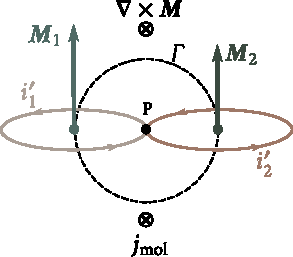
\includegraphics[scale=1]{figures/ch_07/fig_7_3.pdf}
		\caption[]{}
		\label{fig:7_3}
	\end{center}
	\vspace{-0.8cm}
\end{figure}

Các dòng điện vi mô $i_1'$ và $i_2'$ chạy trong vòng kín được minh họa ở \fig{7_3} bởi các đường nét liền có thể được coi như độ từ hóa $\vec{M}_1$ và $\vec{M}_2$.
Các vòng này chạy trong mặt phẳng vuông góc với mặt phẳng hình vẽ.
Nếu chiều của vector $\vec{M}_1$ và $\vec{M}_2$ giống nhau, hướng của các dòng $i_1'$ và $i_2'$ tại điểm P sẽ đối nghịch nhau.
Do $M_1=M_2$ nên các dòng $i_1'$ và $i_2'$ có độ lớn bằng nhau, dẫn tới hệ quả là tổng các dòng điện vi mô tại điểm P, giống như $\curlop{\vec{M}}$, bằng không: $\ab{\vec{j}}{mol}=0$.

Giờ ta giả sử rằng $M_1>M_2$.
Khi đó, lưu số của $\vec{M}$ quanh vòng kín $\Gamma$ sẽ khác không và trường vector $\vec{M}$ tại điểm P sẽ được đặc trưng bởi vector $\curlop{\vec{M}}$ hướng ra ngoài mặt phẳng hình vẽ và ra xa chúng ta.
Dòng vi mô lớn hơn ứng với độ từ hóa cao hơn; vậy, trong trường hơp này ta có $i_1'>i_2'$.
Hệ quả là tại điểm P sẽ xuất hiện một dòng điện tổng khác không và được đặc trưng bởi mật độ dòng $\ab{\vec{j}}{mol}$.
Đại lượng này cũng hướng ra xa chúng ta tương tự $\curlop{\vec{M}}$, .
Khi $M_1<M_2$, các vector $\curlop{\vec{M}}$ and $\ab{\vec{j}}{mol}$ sẽ hướng tới chúng ta thay vì hướng ra ngoài.

Vậy ta thấy rằng các vector $\curlop{\vec{M}}$ và $\ab{\vec{j}}{mol}$ có cùng chiều [xem \eqn{7_6}] và tại các điểm mà curl của độ từ hóa khác không, mật độ dòng vi mô sẽ khác không.

Thay \eqn{7_6} cho mật độ dòng vi mô vào \eqn{7_4}:
\begin{equation*}
    \curlop{\vec{B}} = \mu_0 \vec{j} + \mu_0 \curlop{\vec{M}}.
\end{equation*}

\noindent
Chia hai vế phương trình cho $\mu_0$ và kết hợp các curl lại, ta được
\begin{equation}\label{eq:7_7}
    \curlop{\parenthesis{\frac{\vec{B}}{\mu_0} - \vec{M}}} = \vec{j}.
\end{equation}

\noindent
Từ đây ta suy ra rằng
\begin{equation}\label{eq:7_8}
    \vec{H} = \frac{\vec{B}}{\mu_0} - \vec{M},
\end{equation}

\noindent
chính là đại lượng thứ cấp chúng ta cần tìm: đại lượng mà curl của nó chỉ phụ thuộc vào các dòng vĩ mô.
Đại lượng này được gọi là \textbf{cường độ từ trường.}

Vậy từ \eqn{7_7}:
\begin{equation}\label{eq:7_9}
    \curlop{\vec{H}} = \vec{j}
\end{equation}

\noindent
(curl của vector $\vec{H}$ bằng với vector của mật độ dòng vĩ mô).

Chúng ta sẽ chọn một vòng kín $\Gamma$ bất kì bao quanh diện tích  $S$ và viết biểu thức sau
\begin{equation*}
    \int_S \curlop{\vec{H}} \ccdot \derivec{S} = \int_S \vec{j} \ccdot \derivec{S}.
\end{equation*}

\noindent
Từ định lý Stokes, ta thấy vế trái của biểu thức trên bằng với lưu số của vector $\vec{H}$ quanh vòng kín $\Gamma$.
Do vậy, ta có:
\begin{equation}\label{eq:7_10}
    \oint_{\Gamma} \vec{H} \ccdot \derivec{l} = \int_S \vec{j} \ccdot \derivec{S}.
\end{equation}

\noindent
Nếu ta đang xét các dòng vĩ mô chảy qua dây dẫn được bao bởi vòng kín, \eqn{7_10} có thể được viết lại dưới dạng sau:
\begin{equation}\label{eq:7_11}
    \oint_{\Gamma} \vec{H} \ccdot \derivec{l} = \sum_k I_k.
\end{equation}

\noindent
Phương trình \eqref{eq:7_10} và \eqref{eq:7_11} giúp biểu diễn định lý về lưu số của the vector $\vec{H}$: \textit{lưu số của vector cường độ từ trường quanh một vòng kín bằng với tổng đại số của các dòng vĩ mô được bao bởi vòng này}.

Cường độ từ trường $\vec{H}$ tương đương với cảm ứng điện trường $\vec{D}$.
It was originally assumed that magnetic masses similar to electric charges exist in nature, and the science of magnetism developed along the lines of that of electricity.
Back in those times, the relevant names were introduced: the ``magnetic induction'' for $\vec{B}$ and the ``field strength'' (formerly ``field intensity'') for $\vec{H}$.
It was later established that no magnetic masses exist in nature and that the quantity called the magnetic induction is actually the analogue not of the electric displacement $\vec{D}$, but of the electric field strength $\vec{E}$ (accordingly, $\vec{H}$ is the analogue of $\vec{D}$ instead of $\vec{E}$).
It was decided not to change the established terminology, however, moreover because owing to the different nature of an electric and a magnetic field (an electrostatic field is potential, a magnetic one is solenoidal\footnote{A solenoidal field is one having no sources. At each point of such a field,
the divergence is zero.}) the quantities $\vec{B}$ and $\vec{D}$ display many similarities in their behaviour (for example, the $\vec{B}$ lines, like the $\vec{D}$ lines, are not disrupted at the interface between two media).

In a vacuum, $\vec{M}=0$, therefore, $\vec{H}$ transforms into $\vec{B}/\mu_0$ and \eqns{7_10}{7_11} transform into \eqns{6_103}{6_101}.

In accordance with \eqn{6_30}, the strength of the field of a line current in a vacuum is determined by the expression
\begin{equation}\label{eq:7_12}
    H = \frac{1}{4\pi}\frac{2I}{b},
\end{equation}

\noindent
whence it can be seen that the magnetic field strength has a dimension equal to that of current divided by that of length.
In this connection, the SI unit of magnetic field strength is called the ampere per metre (\si{\ampere\per\metre}).

In the Gaussian system, the magnetic field strength is defined as the quantity
\begin{equation}\label{eq:7_13}
    \vec{H} = \vec{B} - 4\pi \vec{M}.
\end{equation}

\noindent
It follows from this definition that in a vacuum $\vec{H}$ coincides with $\vec{B}$.
Accordingly, the unit of $\vec{H}$ in the Gaussian system, called the \textbf{oersted} (\si{\oersted}), has the same value and dimension as the unit of magnetic induction---the gauss (\si{\gauss}).
In essence, the oersted and gauss are different names of the same unit.
If the latter measures $\vec{H}$, it is called the oersted, and if it measures $\vec{B}$, the gauss.

It is customary practice to associate the magnetization not with the magnetic induction, but with the field strength.
It is assumed that at every point of a magnetic
\begin{equation}\label{eq:7_14}
    \vec{M} = \ab{\chi}{m} \vec{H},
\end{equation}

\noindent
where $\ab{\chi}{m}$ is a quantity characteristic of a given magnetic and called the \textbf{magnetic susceptibility}\footnote{In anisotropic media, the directions of the vectors $\vec{M}$ and $\vec{H}$, generally speaking, do not coincide. For such media, the relatiom between the vectors $\vec{M}$ and $\vec{H}$ is achieved by means of the \textbf{magnetic susceptibility tensor} (see the footnote number 2 on page 55).}.
Experiments show that for weakly magnetic (non-ferromagnetic) substances in not too strong fields
$\ab{\chi}{m}$ is independent of $\vec{H}$.
According to \eqn{7_8}, the dimension of $\vec{H}$ coincides with that of $\vec{M}$.
Hence, $\ab{\chi}{m}$ is a dimensionless quantity.

Using \eqn{7_14} for $\vec{M}$ in \eqn{7_8}, we get
\begin{equation*}
    \vec{H} = \frac{\vec{B}}{\mu_0} - \ab{\chi}{m} \vec{H},
\end{equation*}

\noindent
whence
\begin{equation}\label{eq:7_15}
    \vec{H} = \frac{\vec{B}}{\mu_0 (1 + \ab{\chi}{m})}.
\end{equation}

The dimensionless quantity
\begin{equation}\label{eq:7_16}
    \mu = 1 + \ab{\chi}{m},
\end{equation}

\noindent
is called the \textbf{relative permeability} or simply the \textbf{permeability} of a substance\footnote{The so-called absolute permeability $\ab{\mu}{a}=\mu_0\mu$ is introduced in electrical engineering. This quantity is deprived of a physical meaning, however, and we shall not use it.}.

Unlike the dielectric susceptibility $\chi$ that can have only positive values (the polarization $\vec{P}$ in an isotropic dielectric is always directed along the $\vec{E}$ field), the magnetic susceptibility $\ab{\chi}{m}$ may be either positive or negative.
Hence, the permeability may be either greater or smaller than unity.

With account taken of \eqn{7_16}, \eqn{7_15} can be written as follows:
\begin{equation}\label{eq:7_17}
    \vec{H} = \frac{\vec{B}}{\mu_0\mu}.
\end{equation}

\noindent
Thus, the magnetic field strength $\vec{H}$ is a vector having the same direction as the vector $\vec{B}$, but whose magnitude is $\mu_0\mu$ times smaller (in anisotropic media the vectors $\vec{H}$ and $\vec{B}$, generally speaking, do not coincide in direction).

Equation \eqref{eq:7_14} relating the vectors $\vec{M}$ and $\vec{H}$ has exactly the same form in the Gaussian system too.
Using this equation in \eqn{7_13}, we get
\begin{equation*}
    \vec{H} = \vec{B} - 4\pi\ab{\chi}{m} \vec{H},
\end{equation*}

\noindent
whence
\begin{equation}\label{eq:7_18}
    \vec{H} = \frac{\vec{B}}{1 + 4\pi\ab{\chi}{m}}.
\end{equation}

The dimensionless quantity
\begin{equation}\label{eq:7_19}
    \mu = 1 + 4\pi\ab{\chi}{m},
\end{equation}

\noindent
is called the \textbf{permeability} of a substance.
Introducing this quantity into \eqn{7_18}, we get
\begin{equation}\label{eq:7_20}
    \vec{H} = \frac{\vec{B}}{\mu}.
\end{equation}

The value of $\mu$ in the Gaussian system of units coincides with its value in the SI.
A comparison of \eqns{7_16}{7_19} shows that the value of the magnetic susceptibility in the SI is $4\pi$ times that of $\ab{\chi}{m}$ in the Gaussian system:
\begin{equation}\label{eq:7_21}
    \ab{\chi}{m,SI} = 4\pi\ab{\chi}{m,Gs}.
\end{equation}

\section{Calculation of the Field in Magnetics}\label{sec:7_3}

Let us consider the field produced by an infinitely long round magnetized rod. We shall consider the magnetization $\vec{M}$ to be the same everywhere and directed along the axis of the rod.
Let us divide the rod mentally into layers of thickness $\deriv{l}$ at right angles to the axis.
We shall divide each layer in turn into small cylindrical elements with bases of an arbitrary shape and of area $\deriv{S}$ (\fig{7_4}a).
Each such element has the magnetic moment
\begin{equation}\label{eq:7_22}
    \deriv{\ab{p}{m}} = M\, \deriv{S}\, \deriv{l}.
\end{equation}

The field $\derivec{B}'$ set up by an element at distances that are great in comparison with its dimensions is equivalent to the field that would produce the current $I=M\,\deriv{l}$ flowing around the element along its side surface (see \fig{7_4}b).
Indeed, the magnetic moment of such a current is $\deriv{\ab{p}{m}}=I\,\deriv{S}=M\,\deriv{l}\,\deriv{S}$ [compare with \eqn{7_22}], while the magnetic field at great distances is determined only by the
magnitude and direction of the magnetic moment (see \sect{6_9}).

\begin{figure}[!htb]
	\begin{center}
		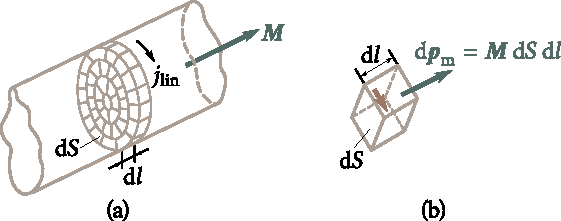
\includegraphics[scale=1]{figures/ch_07/fig_7_4.pdf}
		\caption[]{}
		\label{fig:7_4}
	\end{center}
	\vspace{-0.8cm}
\end{figure}

The imaginary currents flowing in the section of the surface common for two adjacent elements are identical in magnitude and opposite in direction, therefore their sum is zero. Thus, when summating the currents flowing around the side surfaces of the elements of one layer, only the currents flowing along the side surface of the layer will remain uncompensated.

It follows from the above that a rod layer of thickness $\deriv{l}$ sets up a field equivalent to the one which would be produced by the current $M\,\deriv{l}$ flowing around the layer along its side surface (the linear density of this current is $\ab{j}{lin}=M$).
The entire infinite magnetized rod sets up a field equivalent to the field of a cylinder around which flows a current having the linear density $\ab{j}{lin}=M$. We established in \sect{6_2} that outside such a cylinder the field vanihes, while inside it the field is homogeneous and equals $\mu_0\ab{j}{lin}$ in magnitude.

We have, thus, determined the nature of the field $\vec{B}'$ set up by a homogeneously magnetized infinitely long round rod.
Outside the rod, the field vanishes.
Inside it, the field is homogeneous and equals
\begin{equation}\label{eq:7_23}
    \vec{B}' = \mu_0 \vec{M}.
\end{equation}

Assume that we have a homogeneous field $\vec{B}_0$ set up by macrocurrents in a vacuum.
According to \eqn{7_17}, the strength of this field is
\begin{equation}\label{eq:7_24}
    \vec{H}_0 = \frac{\vec{B}_0}{\mu_0}.
\end{equation}

\noindent
Let us introduce into this field (we shall call it an external one) an infinitely long round rod of a homogeneous and isotropic magnetic, arranging it along the direction of $\vec{B}_0$.
It follows from considerations of symmetry that the magnetization $\vec{M}$ set up in the rod is collinear with the vector $\vec{B}_0$.

The magnetized rod produces inside itself the field $\vec{B}'$ determined by \eqn{7_23}.
The field inside the rod, as a result, becomes equal to
\begin{equation}\label{eq:7_25}
    \vec{B} = \vec{B}_0 + \vec{B}' = \vec{B}_0 + \mu_0 \vec{M}.
\end{equation}

\noindent
Using this value of $\vec{B}$ in \eqn{7_8}, we get the strength of the field inside the rod
\begin{equation*}
    \vec{H} = \frac{\vec{B}}{\mu_0} - \vec{M} = \frac{\vec{B}_0}{\mu_0} = \vec{H}_0
\end{equation*}

\noindent
[see \eqn{7_24}]. Thus, the strength of the field in the rod coincides with that of the external field.

Multiplying $\vec{H}$ by $\mu_0\mu$ we get the magnetic induction inside the rod:
\begin{equation}\label{eq:7_26}
    \vec{B} = \mu_0\mu\vec{H} = \mu_0\mu \frac{\vec{B}_0}{\mu_0} = \mu \vec{B}_0.
\end{equation}

\noindent
Hence, it follows that the permeability $\mu$ shows how many times the field increases in a magnetic [compare with \eqn{7_26}].

It must be noted that since the field $\vec{B}'$ is other than zero only inside the rod, the magnetic field outside the rod remains unchanged.

The result we have obtained is correct when a homogeneous and isotropic magnetic fills the volume bounded by surfaces formed by the strength lines of the external field\footnote{We remind our reader that for an electric field $\vec{D} = \vec{D}_0$ provided that a homogeneous and isotropic dielectric fills the volume bounded by equipotential surfaces, \ie, surfaces orthogonal to the strength lines of the external field.}.
Otherwise, the field strength determined by \eqn{7_8} does not coincide with $\vec{H}_0=\vec{B}_0/\mu_0$.

It is conditionally assumed that the field strength in a magnetic is
\begin{equation}\label{eq:7_27}
    \vec{H} = \vec{H}_0 - \ab{\vec{H}}{d},
\end{equation}

\noindent
where $\vec{H}_0$ is the external field, and $\ab{\vec{H}}{d}$ is the so-called \textbf{demagnetizing field}.
The latter is assumed to be proportional to the magnetization
\begin{equation}\label{eq:7_28}
    \ab{\vec{H}}{d} = N \vec{M}.
\end{equation}

\noindent
The proportionality constant $N$ is known as the \textbf{demagnetization factor}.
It depends on the shape of a magnetic.
We have seen that $\vec{H} = \vec{H}_0$ for a body whose surface is not intersected by strength lines of the external field, \ie, the demagnetization factor is zero.
For a thin disk perpendicular to the external field, $N = 1$, and for a sphere, $N = 1/3$.

The relevant calculations show that when a homogeneous and isotropic magnetic having the shape of an ellipsoid is placed in a homogeneous external field, the magnetic field in it is also homogeneous, although it differs from the external one.
This also holds for a sphere, which is a particular case of an ellipsoid, and for a long rod and a thin disk, which can be considered as the extreme cases of an ellipsoid.

In concluding, let us find the field strength of an infinitely long solenoid filled with a homogeneous and isotropic magnetic (or submerged in an infinite homogeneous and isotropic magnetic.).
Applying the theorem on circulation [see \eqn{7_11}] to the loop shown in \fig{6_30}, we get the equation $Ha = naI$.
Hence,
\begin{equation}\label{eq:7_29}
    H = nI.
\end{equation}

\noindent
Thus, the field strength inside an infinitely long solenoid equals the product of the current and the number of turns per unit length.
Outside the solenoid, the field strength vanishes.

\section{Conditions at the Interface of Two Magnetics}\label{sec:7_4}

Near the interface of two magnetics, the vectors $\vec{B}$ and $\vec{H}$ must comply with definite boundary conditions that follow from the relations
\begin{equation}\label{eq:7_30}
    \divop{\vec{B}} = 0,\quad \curlop{\vec{H}} = \vec{j}
\end{equation}

\noindent
[see \eqns{7_3}{7_9}].
We are considering stationary fields, \ie, ones that do not vary with time.

Let us take on the interface of two magnetics of permeabilities $\mu_1$ and $\mu_2$ an imaginary cylindrical surface of height $h$ with bases $S_1$ and $S_2$ at different sides of the interface (\fig{7_5}).
The flux of the vector $\vec{B}$ through this interface is
\begin{equation}\label{eq:7_31}
    \Phi_B = \ab{B}{$1$,n} S + \ab{B}{$2$,n} S + \average{\ab{B}{n}} \ab{S}{side}
\end{equation}

\noindent
[compare with \eqn{2_46}].

Since $\divop{\vec{B}}=0$, the flux of the vector $\vec{B}$ through any closed surface is zero.
Equating expression \eqref{eq:7_31} to zero and making the transition $h\to 0$, we arrive at the equation $\ab{B}{$1$,n}=-\ab{B}{$2$,n}$.
If we project $\vec{B}_1$ and $\vec{B}_2$ onto the same normal, we get the condition
\begin{equation}\label{eq:7_32}
    \ab{B}{$1$,n} = \ab{B}{$2$,n}
\end{equation}

\noindent
[compare with \eqn{2_47}].

Replacing in accordance with \eqn{7_17} the components of $\vec{B}$ with the corresponding components of $\vec{H}$ multiplied by $\mu_0\mu$, we get the equation
\begin{equation*}
    \mu_0\mu_1 \ab{H}{$1$,n} = \mu_0\mu_2 \ab{H}{$2$,n},
\end{equation*}

\noindent
whence
\begin{equation}\label{eq:7_33}
    \frac{\ab{H}{$1$,n}}{\ab{H}{$2$,n}} = \frac{\mu_2}{\mu_1}.
\end{equation}

\begin{figure}[!htb]
	\begin{minipage}[t]{0.48\linewidth}
		\begin{center}
			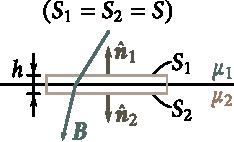
\includegraphics[scale=1]{figures/ch_07/fig_7_5.pdf}
			\caption[]{}
			\label{fig:7_5}
		\end{center}
	\end{minipage}
	\hfill{ }%space{-0.05cm}
	\begin{minipage}[t]{0.48\linewidth}
		\begin{center}
			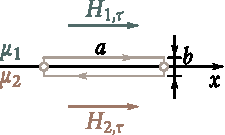
\includegraphics[scale=1]{figures/ch_07/fig_7_6.pdf}
			\caption[]{}
			\label{fig:7_6}
		\end{center}
	\end{minipage}
\vspace{-0.4cm}
\end{figure}

Now let us take a rectangular loop on the interface of the magnetics (\fig{7_6}) and calculate the circulation of $\vec{H}$ for it.
With small dimensions of the loop, the circulation can be written in the form
\begin{equation}\label{eq:7_34}
    \oint H_l\, \deriv{l} = H_{1,\tau} a - H_{2,\tau} a + \average{H_l} 2b,
\end{equation}

\noindent
where $\average{H_l}$ is the average value of $\vec{H}_l$ on the parts of the loop at right angles to the interface.
If no macroscopic currents flow along the interface of the magnetics, $\curlop{\vec{H}}$ within the limits of the loop will equal zero.
Consequently, the circulation will also be zero.
Assuming that \eqn{7_34} is zero and performing the limit transition $b\to 0$, we arrive at the expression
\begin{equation}\label{eq:7_35}
    H_{1,\tau} = H_{2,\tau}
\end{equation}

\noindent
[compare with \eqn{2_44}].

Replacing the components of $\vec{H}$ with the corresponding components of $\vec{B}$ divided by $\mu_0\mu$, we get the relation
\begin{equation*}
    \frac{B_{1,\tau}}{\mu_0\mu_1} = \frac{B_{2,\tau}}{\mu_0\mu_2},
\end{equation*}

\noindent
whence it follows that
\begin{equation}\label{eq:7_36}
    \frac{B_{1,\tau}}{B_{2,\tau}} = \frac{\mu_1}{\mu_2}.
\end{equation}

Summarizing, we can say that in passing through the interface between two magnetics, the normal component of the vector $\vec{B}$ and the tangential component of the vector $\vec{H}$ change continuously.

The tangential component of the vector $\vec{B}$ and the normal component of the vector $\vec{H}$ in passing through the interface of the magnetics, however, experience a discontinuity.
Thus, when passing through the interface of two media, the vector $\vec{B}$ behaves similar to the vector $\vec{D}$, and the vector $\vec{H}$ similar to the vector $\vec{E}$.

Figure \ref{fig:7_7} shows the behaviour of the $\vec{B}$ lines when intersecting the surface between two magnetics.
Let the angles between the $\vec{B}$ lines and a normal to the interface be $\alpha_1$ and $\alpha_2$, respectively.
The ratio of the tangents of these angles is
\begin{equation*}
    \frac{\tan{\alpha_1}}{\tan{\alpha_2}} = \frac{B_{1,\tau}/\ab{B}{$1$,n}}{B_{2,\tau}/\ab{B}{$2$,n}},
\end{equation*}

\noindent
whence with a view to \eqns{7_32}{7_36} we get a law of refraction of the magnetic field lines similar to \eqn{2_49}:
\begin{equation}\label{eq:7_37}
    \frac{\tan{\alpha_1}}{\tan{\alpha_2}} = \frac{\mu_1}{\mu_2}.
\end{equation}

\begin{figure}[!htb]
	\begin{center}
		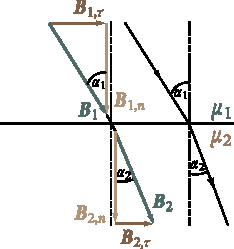
\includegraphics[scale=1.1]{figures/ch_07/fig_7_7.pdf}
		\caption[]{}
		\label{fig:7_7}
	\end{center}
	\vspace{-0.8cm}
\end{figure}

Upon passing into a magnetic with a greater value of $\mu$, the magnetic field lines deviate from a normal to the surface.
This leads to crowding of the lines.
The crowding of the $\vec{B}$ lines in a substance with a great permeability makes it possible to form magnetic beams, \ie, impart the required shape and direction to them.
In particular, for magnetic shielding of a space, it is surrounded with an iron screen.
A glance at \fig{7_8} shows that the crowding of the magnetic field lines in the body of the screen results in weakening of the field inside it.

Figure \ref{fig:7_9} is a schematic view of a laboratory electromagnet.
It consists of an iron core onto which coils supplied with a current are fitted.
The magnetic field lines are mainly concentrated inside the core.
Only in the narrow air gap do they pass in a medium with a low value of $\mu$.
The vector $\vec{B}$ intersects the boundaries between the air gap and the core along a normal to the interface.
It thus follows, in accordance with \eqn{7_32}, that the magnetic induction in the gap and in the core is identical in value.
Let us apply the theorem on the circulation of $\vec{H}$ to the loop along the axis of the core.
We can assume that the field strength is identical everywhere in the iron and is $\ab{H}{iron} = B/(\mu_0\ab{\mu}{iron})$.
In the air, $\ab{H}{air} = B/(\mu_0\ab{\mu}{air})$.
Let us denote the length of the loop section in the iron by $\ab{l}{iron}$ and in the gap by $\ab{l}{air}$.
The Circulation can, thus, be written in the form
$\ab{H}{iron}\ab{l}{iron} + \ab{H}{air}\ab{l}{air}$.
According to \eqn{7_11}, this circulation must equal
$NI$, where $N$ is the total number of turns of the electromagnet coils, and $I$ is the current.
Thus,
\begin{equation*}
    \frac{B}{\mu_0\ab{\mu}{iron}} \ab{l}{iron} + \frac{B}{\mu_0\ab{\mu}{air}} \ab{l}{air} = NI.
\end{equation*}

\noindent
Hence,
\begin{equation*}
    B = \mu_0 I \frac{N}{\parenthesis{\dfrac{\ab{l}{air}}{\ab{\mu}{air}} + \dfrac{\ab{l}{iron}}{\ab{\mu}{iron}}}} \approx \mu_0 I \frac{N}{\parenthesis{\ab{l}{air} + \dfrac{\ab{l}{iron}}{\ab{\mu}{iron}}}}
\end{equation*}

\noindent
($\ab{\mu}{air}$ differs from unity only in the fifth digit after the decimal point).

\begin{figure}[!htb]
	\begin{minipage}[t]{0.48\linewidth}
		\begin{center}
			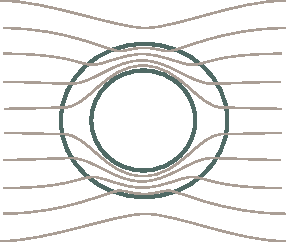
\includegraphics[scale=1]{figures/ch_07/fig_7_8.pdf}
			\caption[]{}
			\label{fig:7_8}
		\end{center}
	\end{minipage}
	\hfill{ }%space{-0.05cm}
	\begin{minipage}[t]{0.48\linewidth}
		\begin{center}
			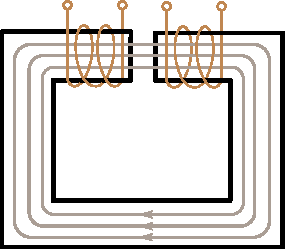
\includegraphics[scale=1]{figures/ch_07/fig_7_9.pdf}
			\caption[]{}
			\label{fig:7_9}
		\end{center}
	\end{minipage}
\vspace{-0.4cm}
\end{figure}

Usually, $\ab{l}{air}$ is of the order of \SI{0.1}{\metre}, $\ab{l}{iron}$ is of the order of \SI{1}{\metre}, while $\ab{\mu}{iron}$ reaches values of the order of several thousands.
We may, therefore, disregard the second addend in the denominator and write that
\begin{equation}\label{eq:7_38}
    B = \mu_0 I \frac{N}{\ab{l}{air}}.
\end{equation}

\noindent
Consequently, the magnetic induction in the gap of an electromagnet has the same value as it would have inside a toroid without a core when $N/\ab{l}{air}$ turns are wound on the torus per unit length [see \eqn{6_110}].
By increasing the total number of turns and reducing the dimensions of the air gap, we can obtain fields with a high value of $B$.
In practice, fields with $B$ of the order of several teslas (several tens of thousands of gausses) are obtained with the aid of electromagnets having an iron core.

\section{Kinds of Magnetics}\label{sec:7_5}

Equation \eqref{eq:7_14} determines the magnetic susceptibility $\ab{\chi}{m}$ of a unit volume of a substance.
This susceptibility is often replaced with the molar (for chemically simple substances---the atomic) susceptibility $\ab{\chi}{m,mol}$ ($\ab{\chi}{m,at}$) related to one mole of a substance.
It is evident that $\ab{\chi}{m,mol} = \ab{\chi}{m} \ab{V}{mol}$, where $\ab{V}{mol}$ is the volume of
a mole of a substance.
Whereas $\ab{\chi}{m}$ is a dimensionless quantity,
$\ab{\chi}{m,mol}$ is measured in \si{\metre\cubed\per\mole}.

Depending on the sign and magnitude of the magnetic susceptibility, all magnetics are divided into three groups:
\begin{enumerate}[(1)]
    \item \textbf{diamagnetics}, for which $\ab{\chi}{m}$ is negative and small in absolute value ($|\ab{\chi}{m,mol}|$ is about \SIrange{e-11}{e-10}{\metre\cubed\per\mole});
    \item \textbf{paramagnetics}, for which $\ab{\chi}{m}$ is also not great, but positive
    ($\ab{\chi}{m,mol}$ is about \SIrange{e-10}{e-10}{\metre\cubed\per\mole});
    \item \textbf{ferromagnetics}, for which $\ab{\chi}{m}$ is positive and reaches very     great values ($\ab{\chi}{m,mol}$ is about \SI{1}{\metre\cubed\per\mole}). In addition, unlike diamagnetics and paramagnetics for which $\ab{\chi}{m}$ does not depend on $H$, the susceptibility of ferromagnetics is a function of the magnetic field strength.
\end{enumerate}

Thus, the magnetization $\vec{M}$ in isotropic substances may either coincide in direction with $\vec{H}$ (in paramagnetics and ferromagnetics), or be directed oppositely to it (in diamagnetics).
We remind our reader that in isotropic dielectrics the polarization is always directed in the same way as $\vec{E}$.

\section{Gyromagnetic Phenomena}\label{sec:7_6}

The nature of molecular currents became clear after the British physicist Ernest Rutherford (1871-1937) established experimentally that the atoms of all substances consist of a positively charged nucleus and negatively charged electrons travelling around it.

The motion of electrons in atoms obeys quantum laws; in particular, the concept of a trajectory cannot be applied to the electrons travelling in an atom.
The diamagnetism of a substance can be explained, however, by using the very simple Bohr model of an atom.
According to this model, the electrons in atoms travel along stationary circular orbits.

\begin{figure}[!htb]
	\begin{center}
		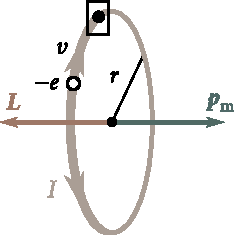
\includegraphics[scale=1]{figures/ch_07/fig_7_10.pdf}
		\caption[]{}
		\label{fig:7_10}
	\end{center}
	\vspace{-0.8cm}
\end{figure}

Assume that an electron is moving with the speed $v$ in an orbit of radius $r$ (\fig{7_10}).
The charge $e\nu$, where $e$ is the charge of an electron and $\nu$ is its number of revolutions a second, will be carried through an area at any place along the path of the electron in one second.
Hence, an electron travelling in orbit will form the ring current $I=e\nu$.
Since the charge of an electron is negative, the direction of motion of the electron and the direction of the current will be opposite.
The magnetic moment of the current set up by an electron is
\begin{equation*}
    \ab{p}{m} = IS = e\nu\pi r^3.
\end{equation*}

\noindent
The product $2\pi r\nu$ gives the speed of the electron $v$, therefore, we can write that
\begin{equation}\label{eq:7_39}
    \ab{p}{m} = \frac{evr}{2}.
\end{equation}

\noindent
The moment \eqref{eq:7_39} is due to the motion of an electron in orbit and is, therefore, called the \textbf{orbital magnetic moment}.
The direction of the vector $\ab{\vec{p}}{m}$ forms a right-handed system with the direction of the current, and a left-handed one with that of motion of the electron (see \fig{7_10}).

An electron moving in orbit has the angular momentum
\begin{equation}\label{eq:7_40}
    L = mvr
\end{equation}

\noindent
($m$ is the mass of an electron). The vector $\vec{L}$ is called the \textbf{orbital angular momentum} of an electron.
It forms a right-handed system with the direction of motion of the electron.
Hence, the vectors $\ab{\vec{p}}{m}$ and $\vec{L}$ are directed oppositely.

The ratio of the magnetic moment of an elementary particle to its angular momentum is called the \textbf{gyromagnetic} (or \textbf{magneto mechanical}) ratio.
For an electron, it is
\begin{equation}\label{eq:7_41}
    \frac{\ab{p}{m}}{L} = - \frac{e}{2m}
\end{equation}

\noindent
($m$ is the mass of an electron; the minus sign indicates that the magnetic moment and the angular momentum are directed oppositely).

Owing to its rotation about the nucleus, an electron is similar to a spinning top or gyroscope.
This circumstance underlies the so-called \textbf{gyromagnetic phenomena} consisting in that the magnetization of a magnetic leads to its rotation, and, conversely, the rotation of a magnetic leads to its magnetization.
The existence of the first phenomenon was proved experimentally by A. Einstein and W. de Haas, and of the second by S. Barnett.

Einstein and de Haas based their experiment on the following reasoning.
If we magnetize a rod made of a magnetic, then the magnetic moments of the electrons will be aligned in the direction of the field and the angular momenta in the opposite direction.
As a result, the total angular momentum of the electrons $\sum_i\vec{L}_i$ will become other than zero (initially owing to the chaotic orientation of the individual momenta it equalled zero).
The angular momentum of the system rod + electrons must remain unchanged.
Therefore, the rod acquires the angular momentum $-\sum_i\vec{L}_i$ and, consequently, begins to rotate.
A change in the direction of magnetization leads to a change in the direction of rotation of the rod.

A mechanical model of this experiment can be carried out by seating a person on a rotatable stool and having him hold a massive rotating wheel in his hands.
When he holds the axle of the wheel upward, he begins to rotate in the direction opposite to that of rotation of the wheel.
When he turns the axle downward, he begins to rotate in the other direction.

\begin{figure}[!htb]
	\begin{center}
		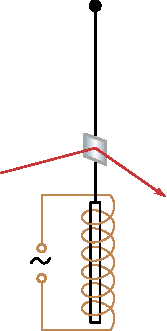
\includegraphics[scale=1]{figures/ch_07/fig_7_11.pdf}
		\caption[]{}
		\label{fig:7_11}
	\end{center}
	\vspace{-0.8cm}
\end{figure}

Einstein and de Haas conducted their experiment as follows (\fig{7_11}).
A thin iron rod was suspended on an elastic thread and placed inside a solenoid.
The thread was twisted very slightly when the rod was magnetized using a constant magnetic field.
The resonance method was used to increase the effect---the solenoid was fed with an alternating current whose frequency was chosen equal to the natural frequency of mechanical oscillations of the system.
In these conditions, the amplitude of the oscillations reached values that could be measured by watching the displacement of a light spot reflected by a mirror fastened to the thread.
The data obtained in the experiment were used to calculate the gyromagnetic ratio, which was found to equal $-(e/m)$.
Thus, the sign of the charge of the carriers setting up the molecular currents coincided with the sign of the charge of an electron.
The result obtained, however, was double the expected value of the gyromagnetic ratio \eqref{eq:7_41}.

To understand Barnett's experiment, we must remember that when an attempt was made to bring a gyroscope into rotation about a certain direction, the gyroscope axis turned so that the directions of the natural and forced rotations of the gyroscope coincided (see Sec. 5.9 of Vol. I).
If we place a gyroscope fastened in a universal joint on the disk of a centrifugal machine and begin to rotate it, the gyroscope axis will align itself vertically, and in such a way that the direction of rotation of the gyroscope will coincide with that of the disk.
When the direction of rotation of the centrifugal machine is reversed, the gyroscope axis will turn through $180$ degrees, \ie, in such a way that the directions of the two rotations will again coincide.

Barnett rotated an iron rod very rapidly about its axis and measured the produced magnetization.
Barnett also obtained a value for the gyromagnetic ratio from the results of his experiment double that given by \eqn{7_41}.

It was discovered later that apart from the orbital magnetic moment \eqref{eq:7_39} and the orbital angular momentum \eqref{eq:7_40}, an electron has its intrinsic angular momentum $\ab{L}{s}$ and magnetic moment $\ab{p}{m,s}$ for which the gyromagnetic ratio is
\begin{equation}\label{eq:7_42}
    \frac{\ab{p}{m,s}}{\ab{L}{s}} = - \frac{e}{m},
\end{equation}

\noindent
\ie, coincides with the value obtained in the experiments conducted by Einstein and de Haas and by Barnett.
It thus follows that the magnetic properties of iron are due not to the orbital, but to the intrinsic magnetic moment of its electrons.

Attempts were initially made to explain the existence of the intrinsic magnetic moment and angular momentum of an electron by considering it as a charged sphere spinning about its axis.
Accordingly, the intrinsic angular momentum of an electron was named its \textbf{spin}.
It was discovered quite soon, however, that such a notion results in a number of contradictions, and it became necessary to reject the hypothesis of a ``spinning'' electron.
It is assumed at present that the intrinsic angular momentum (spin) and the intrinsic (spin) magnetic moment associated with it are inherent properties of an electron like its mass and charge.

Not only electrons, but also other elementary particles have a spin.
The spin\footnote{More exactly, the maximum value of the projection of the spin onto a direction separated in space, for example, onto that of the extenal field.} of elementary particles is an integral or half-integral multiple of the quantity $\hslash$ equal to Planck's constant $h$ divided by $2\pi$
\begin{equation}\label{eq:7_43}
    \hslash = \frac{h}{2\pi} = \SI{1.05e-34}{\joule\second} = \SI{1.05e-2}{\erg\second}.
\end{equation}

\noindent
In particular, for an electron, $\ab{L}{s}=\hslash/2$; in this connection, the spin of an electron is said to equal $1/2$.
Thus, $\hslash$ is a natural unit of the angular momentum like the elementary charge $e$ is a natural unit of charge.

In accordance with \eqn{7_42}, the intrinsic magnetic moment of an electron is
\begin{equation}\label{eq:7_44}
    \ab{p}{m} = - \frac{e}{m} \ab{L}{s} = - \frac{e}{m} \frac{\hslash}{2} = - \frac{e\hslash}{2m}.
\end{equation}

\noindent
The quantity\footnote{According to the equation $W=-\ab{\vec{p}}{m}\ccdot\vec{B}$, the dimension of magnetic moment equals that of energy (joule or erg) divided by the dimension of magnetic induction (tesla or gauss).}
\begin{equation}\label{eq:7_45}
    \ab{\mu}{B} = \frac{e\hslash}{2m} = \SI{0.927e-23}{\joule\per\tesla} = \SI{0.927e-20}{\erg\per\gauss}
\end{equation}

\noindent
is called the \textbf{Bohr magneton}.
Hence, the intrinsic magnetic moment of an electron equals one Bohr magneton.

The magnetic moment of an atom consists of the orbital and intrinsic moments of the electrons in it, and also of the magnetic moment of the nucleus (which is due to the magnetic moments of the elementary particles---protons and neutrons---forming
the nucleus).
The magnetic moment of a nucleus is much smaller than
the moments of the electrons.
For this reason, they may be disregarded when considering many questions, and we may consider the magnetic moment of an atom to equal the vector sum of the magnetic moments of its electrons.
The magnetic moment of a molecule may also be considered equal to the sum of the magnetic moments of all its electrons.

0. Stern and W. Gerlach determined the magnetic moments of atoms experimentally.
They passed a beam of atoms through a greatly inhomogeneous magnetic field.
The inhomogeneity of the field was achieved by using a special shape of the electromagnet pole shoes (\fig{7_12}).
By \eqn{6_77}, the atoms of the beam must experience the force
\begin{equation*}
    F = \ab{p}{m} \diffpartial{B}{x} \cos\alpha,
\end{equation*}

\noindent
whose magnitude and sign depend on the angle $\alpha$ made by the vector $\ab{\vec{p}}{m}$ with the direction of the field.
When the moments of the atoms are distributed chaotically by directions, the beam contains particles for which the values of $\alpha$ vary within the limits from $0$ to $\pi$.
It was assumed accordingly that a narrow beam of atoms after passing between the poles would form on a screen a continuous extended trace whose edges would correspond to atoms having orientations at angles of $\alpha=0$ and $a=\pi$ (\fig{7_13}).
The experiment gave unexpected results.
Instead of a continuous extended trace, separate lines were obtained that were arranged symmetrically with respect to the trace of the beam obtained in the absence of a field.

\begin{figure}[!htb]
	\begin{minipage}[t]{0.45\linewidth}
		\begin{center}
			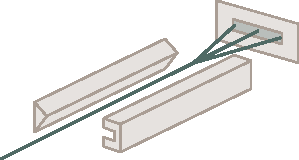
\includegraphics[scale=1]{figures/ch_07/fig_7_12.pdf}
			\caption[]{}
			\label{fig:7_12}
		\end{center}
	\end{minipage}
	\hfill{ }%space{-0.05cm}
	\begin{minipage}[t]{0.52\linewidth}
		\begin{center}
			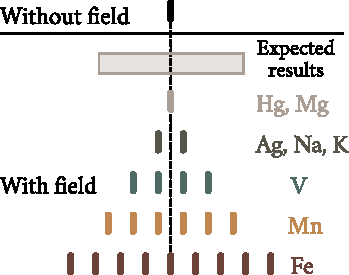
\includegraphics[scale=1]{figures/ch_07/fig_7_13.pdf}
			\caption[]{}
			\label{fig:7_13}
		\end{center}
	\end{minipage}
\vspace{-0.4cm}
\end{figure}

The Stern-Gerlach experiment showed that the angles at which the magnetic moments of atoms are oriented relative to a magnetic field can have only discrete values, \ie, that the projection of a magnetic moment onto the direction of a field is quantized.

The number of possible values of the projection of the magnetic moment onto the direction of the magnetic field for different atoms is different.
It is two for silver, aluminium, copper, and the alkali metals, four for vanadium, nitrogen, and the halogens, five for oxygen, six for manganese, nine for iron, ten for cobalt, etc.

Measurements gave values of the order of several Bohr magnetons for the magnetic moments of atoms.
Some atoms showed no deflections (see, for example, the trace of mercury and magnesium atoms in \fig{7_13}), which indicates that they have no magnetic moment.

\section{Diamagnetism}\label{sec:7_7}

An electron travelling in an orbit is like a spinning top.
Therefore, all the features of behaviour of gyroscopes under the action of external forces must be inherent in it, in particular, precession of the electron orbit must appear in the appropriate conditions.
The conditions needed for precession appear if an atom is in an external magnetic field $\vec{B}$ (\fig{7_14}).
In this case, the torque $\vec{T} = \ab{\vec{p}}{m}\times\vec{B}$ is exerted on the orbit.
It tends to set up the orbital magnetic moment of an electron $\ab{\vec{p}}{m}$ in the direction of the field (the angular momentum $\vec{L}$ will be set np against the field).
The torque $\vec{T}$ causes the vectors $\ab{\vec{p}}{m}$ and $\vec{L}$ to precess about the direction of the magnetic induction vector $\vec{B}$ whose velocity is simple to find (see Sec. 5.9 of Vol. I).

During the time $\deriv{t}$, the vector $\vec{L}$ receives the increment $\derivec{L}$ equal to
\begin{equation*}
    \derivec{L} = \vec{T}\, \deriv{t}.
\end{equation*}

\noindent
The vector $\derivec{L}$ like the vector $\vec{T}$, is perpendicular to the plane passing through the vectors $\vec{B}$ and $\vec{L}$; its magnitude is
\begin{equation*}
    |\derivec{L}| = \ab{p}{m} B \sin\alpha\, \deriv{t},
\end{equation*}

\noindent
where $\alpha$ is the angle between $\ab{\vec{p}}{m}$ and $\vec{B}$.

\begin{figure}[!htb]
	\begin{center}
		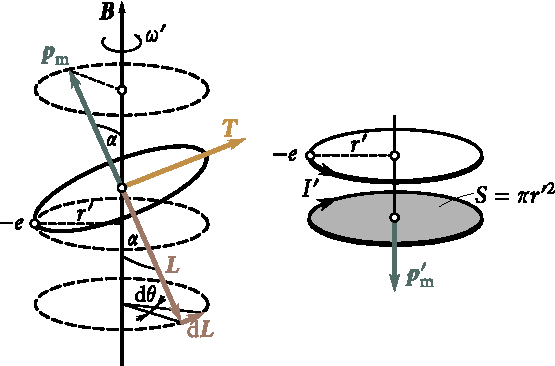
\includegraphics[scale=1]{figures/ch_07/fig_7_14.pdf}
		\caption[]{}
		\label{fig:7_14}
	\end{center}
	\vspace{-0.8cm}
\end{figure}

During the time $\deriv{t}$, the plane containing the vector $\vec{L}$ will turn about the direction of $\vec{B}$ through the angle
\begin{equation*}
    \deriv{\theta} = \frac{|\deriv{L}|}{L\sin\alpha} = \frac{\ab{p}{m}B\sin\alpha\, \deriv{t}}{L\sin\alpha} = \frac{\ab{p}{m}}{L} B\, \deriv{t}.
\end{equation*}

\noindent
Dividing this angle by the time $\deriv{t}$, we find the angular velocity of precession
\begin{equation*}
    \ab{\omega}{L} = \diff{\theta}{t} = \frac{\ab{p}{m}}{L} B.
\end{equation*}

\noindent
Introducing the value of the ratio of the magnetic moment and angular momentum from \eqn{7_41}, we get
\begin{equation}\label{eq:7_46}
    \ab{\omega}{L} = \frac{eB}{2m}.
\end{equation}

The frequency \eqref{eq:7_46} is called the \textbf{frequency of Larmor precession}
or simply the \textbf{Larmor frequency}.
It depends neither on the angle of inclination of an orbit with respect to the direction of the magnetic field nor on the radius of the orbit or the speed of the electron, and, consequently, is the same for all the electrons in an atom.

The precession of an orbit causes additional motion of the electron about the direction of the field.
If the distance $r'$ from the electron to an axis parallel to $\vec{B}$ and passing through the centre of the orbit did not change, the additional motion of the electron would occur along a circle of radius $r'$ (see the unshaded circle in the right part of \fig{7_14}).
The ring current $I' = e (\ab{\omega}{L}/2\pi)$ (see the shaded circle) would correspond to it.
The magnetic moment of this current is
\begin{equation}\label{eq:7_47}
    \ab{p}{m}' = I' S' = e \frac{\ab{\omega}{L}}{2\pi} \pi r'^2 = \frac{e\ab{\omega}{L}}{2} r'^2,
\end{equation}

\noindent
and is directed oppositely to $\vec{B}$ (see the figure). It is called the \textbf{induced magnetic moment}.

Indeed, owing to the motion of an electron in its orbit, the distance $r'$ constantly changes.
Therefore, in \eqn{7_47}, we must replace $r'^2$ with its average value in time $\average{r'^2}$.
The latter depends on the angle $\alpha$ characterizing the orientation of the orbit plane relative to $\vec{B}$.
In particular, for an orbit perpendicular to the vector $\vec{B}$, the quantity $r'$ is constant and equals the radius of the orbit $r$.
For an orbit whose plane passes through the direction of $\vec{B}$, the quantity $r'$ varies according to the law $r' = r\sin(\omega t)$, where $\omega$ is the angular velocity of revolution of an electron in its orbit (\fig{7_15}; the vector $\vec{B}$ and the orbit are in the plane of the drawing).
Consequently, $\average{r'^2}=\average{r^2\sin^2(\omega t)} = r^2/2$ (the quantity $\average{\sin^2(\omega t)}=1$).
Averaging over all possible values of $\alpha$, considering them to be equally probable, yields
\begin{equation}\label{eq:7_48}
    \average{r'^2} = \frac{2}{3} r^2.
\end{equation}

\begin{figure}[!htb]
	\begin{center}
		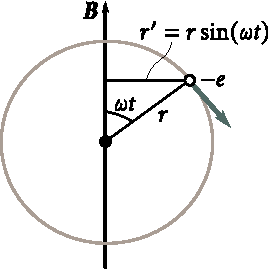
\includegraphics[scale=1]{figures/ch_07/fig_7_15.pdf}
		\caption[]{}
		\label{fig:7_15}
	\end{center}
	\vspace{-0.8cm}
\end{figure}

Using in \eqn{7_47} the value \eqref{eq:7_46} for $\ab{\omega}{L}$ and \eqref{eq:7_48} for $\average{r'^2}$, we get the following expression for the average value of the induced magnetic moment of one electron:
\begin{equation}\label{eq:7_49}
    \average{\ab{p}{m}'} = - \frac{e^2}{6m}r^2 B
\end{equation}

\noindent
(the minus sign reflects the circumstance that the vectors $\average{\ab{\vec{p}}{m}'}$ and $\vec{B}$ have opposite directions).
We assumed the orbit to be circular.
In the general case (for example, for an elliptical orbit), we must take $\average{r^2}$ instead of $r^2$, \ie, the mean square of the distance from an electron to the nucleus.

Summation of \eqn{7_49} over all the electrons yields the induced magnetic moment of an atom
\begin{equation}\label{eq:7_50}
    \ab{p}{m,at}' = \sum \average{\ab{p}{m}'} = - \frac{e^2 B}{6m} \sum_{k=1}^Z \average{r^2_k}
\end{equation}

\noindent
($Z$ is the atomic number of a chemical element; the number of electrons in an atom is $Z$).

Thus, the action of an external magnetic field sets up precession of the electron orbits with the same angular velocity \eqref{eq:7_46} for all the electrons.
The additional motion of the electrons due to precession leads to the production of an induced magnetic moment of an atom [\eqn{7_50}] directed against the field.
Larmor precession appears in all substances without exception.
When atoms by themselves have a magnetic moment, however, a magnetic field not only induces the moment \eqref{eq:7_50}, but also has an orienting action on the magnetic moments of atoms, aligning them in the direction of the field.
The positive (\ie, directed along the field) magnetic moment that appears may be considerably greater than the negative induced moment.
The resultant moment is, therefore, positive and the substance behaves like a paramagnetic.

Diamagnetism is found only in substances whose atoms have no magnetic moment (the vector sum of the orbital and spin magnetic moments of the atom electrons is zero).
If we multiply \eqn{7_50} by the Avogadro constant $\ab{N}{A}$ for such a substance, we get the magnetic moment for a mole of the substance.
Dividing it by the field strength $H$, we find the molar magnetic susceptibility $\ab{\chi}{m,mol}$.
The permeability of dielectrics virtually equals unity.
We can therefore assume that $B/H = \mu_0$.
Thus,
\begin{equation}\label{eq:7_51}
    \ab{\chi}{m,mol} = \frac{\ab{N}{A}\ab{p}{m,at}'}{H} = - \frac{\mu_0 \ab{N}{A} e^2}{6m} \sum_{k=1}^Z \average{r^2_k}.
\end{equation}

\noindent
We must note that the strict quantum-mechanical theory gives exactly the same expression.

Introduction of the numerical values of $\mu_0$, $\ab{N}{A}$, $e$ and $m$ in \eqn{7_51} yields
\begin{equation*}
    \ab{\chi}{m,mol} = -\num{3.55e9} \sum_{k=1}^Z \average{r^2_k}.
\end{equation*}

\noindent
The radii of electron orbits have a value of the order of \SI{e-10}{\metre}.
Hence, the molar diamagnetic susceptibility of the order of \num{e-11} to \num{e-10} is obtained, which agrees quite well with experimental data.

\section{Paramagnetism}\label{sec:7_8}

If the magnetic moment $\ab{p}{m}$ of the atoms differs from zero, the relevant substance is paramagnetic.
A magnetic field tends to align the magnetic moments of the atoms along $\vec{B}$, while thermal motion tends to scatter them uniformly in all directions.
As a result, a certain preferential orientation of the moments is established along the field.
Its value grows with increasing $\vec{B}$ and diminishes with increasing temperature.

The French physicist and chemist Pierre Curie (1859-1906) established experimentally a law (named \textbf{Curie's law} in his honour) according to which the susceptibility of a paramagnetic is
\begin{equation}\label{eq:7_52}
    \ab{\chi}{m,mol} = \frac{C}{T},
\end{equation}

\noindent
where $C$ is the Curie constant depending on the kind of substance and $T$ the absolute temperature.

The classical theory of paramagnetism was developed by the French physicist Paul Langevin (1872-1946) in 1905.
We shall limit ourselves to a treatment of this theory for not too strong fields and not very low temperatures.

According to \eqn{6_76}, an atom in a magnetic field has the potential energy $W=-\ab{p}{m}B\cos\theta$ that depends on the angle $\theta$ between the vectors $\ab{\vec{p}}{m}$ and $\vec{B}$.
Therefore, the equilibrium distribution of the moments by directions must obey Boltzmann's law (see
Sec. 11.8 of Vol. I).
According to this law, the probability of the fact that the magnetic moment of an atom will make with the direction of the vector $\vec{B}$ an angle within the limits from $\theta$ to $\theta+\deriv{\theta}$ is proportional to
\begin{equation*}
    \exp\parenthesis{-\frac{W}{kT}} = \exp\parenthesis{\frac{\ab{p}{m} B \cos\theta}{kT}}.
\end{equation*}

\noindent
Introducing the notation
\begin{equation}\label{eq:7_53}
    a = \frac{\ab{p}{m} B}{kT},
\end{equation}

\noindent
we can write the expression determining the probability in the form
\begin{equation}\label{eq:7_54}
    \exp(a\cos\theta).
\end{equation}

In the absence of a field, all the directions of the magnetic moments are equally probable.
Consequently, the probability of the fact that the direction of a moment will form with a certain direction $z$ an angle within the limits from $\theta$ to $\theta + \deriv{\theta}$ is
\begin{equation}\label{eq:7_55}
    (\deriv{P_{\theta}})_{B=0} = \diff{\Omega_{\theta}}{4\pi} = \frac{2\pi\sin\theta\, \deriv{\theta}}{4\pi} = \frac{1}{2}\sin\theta\, \deriv{\theta}.
\end{equation}

\noindent
Here, $\deriv{\Omega_{\theta}}=2\pi\sin\theta\, \deriv{\theta}$ is the solid angle enclosed between cones having apex angles of $\theta$ and $\theta+\deriv{\theta}$ (\fig{7_16}).

When a field is present, the multiplier \eqref{eq:7_54} appears in the expression for the
probability:
\begin{equation}\label{eq:7_56}
    \deriv{P_{\theta}} = A\, \exp(a\cos\theta) \frac{1}{2}\sin\theta\, \deriv{\theta}
\end{equation}

\noindent
($A$ is a proportionality constant that is meanwhile unknown).

\begin{figure}[!htb]
	\begin{center}
		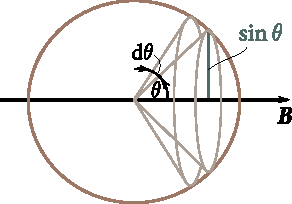
\includegraphics[scale=1]{figures/ch_07/fig_7_16.pdf}
		\caption[]{}
		\label{fig:7_16}
	\end{center}
	\vspace{-0.8cm}
\end{figure}

The magnetic moment of an atom has a magnitude of the order of one Bohr magneton, \ie, about \SI{e-23}{\joule\per\tesla} [see \eqn{7_45}].
At the usually achieved fields, the magnetic induction is of the order of \SI{1}{\tesla} (\SI{e4}{\gauss}).
Hence, $\ab{p}{m}B$ is of the order of \SI{e-23}{\joule}.
The quantity $kT$ at room temperature is about \SI{4e-21}{\joule}.
Thus, $a=\ab{p}{m}B/(kT)$ is much smaller than unity, and $\exp(a\cos\theta)$ may be replaced with the approximate expression $1+a\cos\theta$.
In this approximation, \eqn{7_56} becomes
\begin{equation*}
    \deriv{P_{\theta}} = A (1+a\cos\theta) \frac{1}{2} \sin\theta\, \deriv{\theta}.
\end{equation*}

The constant $A$ can be found by proceeding from the fact that the sum of the probabilities of all possible values of the angle $\theta$ must equal unity:
\begin{equation*}
    1 = \int_0^{\pi} A (1+a\cos\theta) \frac{1}{2} \sin\theta\, \deriv{\theta}.
\end{equation*}

\noindent
Hence, $A=1$, so that
\begin{equation*}
    \deriv{P_{\theta}} = (1+a\cos\theta) \frac{1}{2} \sin\theta\, \deriv{\theta}.
\end{equation*}

Assume that unit volume of a paramagnetic contains $n$ atoms.
Consequently, the number of atoms whose magnetic moments form angles from $\theta$ to $\theta+\deriv{\theta}$ with the direction of the field will be
\begin{equation*}
    \deriv{n_{\theta}} = n\, \deriv{P_{\theta}} = n (1+a\cos\theta) \frac{1}{2} \sin\theta\, \deriv{\theta}.
\end{equation*}

\noindent
Each of these atoms makes a contribution of $\ab{p}{m}\cos\theta$ to the resultant magnetic moment.
Therefore, we get the following expression for the magnetic moment of unit volume (\ie, for the magnetization):
\begin{equation*}
    M = \int_0^{\pi} \ab{p}{m}\cos\theta\, \deriv{n_{\theta}} = \frac{1}{2} n\ab{p}{m} \int_0^{\pi} (1+a\cos\theta) \frac{1}{2} \sin\theta\, \deriv{\theta} = \frac{n\ab{p}{m}a}{3}.
\end{equation*}

\noindent
Substitution for $a$ of its value from \eqn{7_53} yields
\begin{equation*}
    M = \frac{n \ab{p}{m}^2 B}{3kT}.
\end{equation*}

\noindent
Finally, dividing $M$ by $H$ and assuming that $B/H = \mu_0$ (for a paramagnetic $\mu$ is virtually equal to unity), we find the susceptibility
\begin{equation}\label{eq:7_57}
    \ab{\chi}{m} = \frac{\mu_0 n \ab{p}{m}^2}{3kT}.
\end{equation}

Substituting the Avogadro constant $\ab{N}{A}$ for $n$, we get an expression the molar susceptibility:
\begin{equation}\label{eq:7_58}
    \ab{\chi}{m,mol} = \frac{\mu_0 \ab{N}{A} \ab{p}{m}^2}{3kT}.
\end{equation}

\noindent
We have arrived at Curie's law.
A comparison of \eqns{7_52}{7_58} gives the following expression for the Curie constant:
\begin{equation}\label{eq:7_59}
    C = \frac{\mu_0 \ab{N}{A} \ab{p}{m}^2}{3k}.
\end{equation}

It must be remembered that \eqn{7_58} has been obtained assuming that $\ab{p}{m}B\ll kT$.
In very strong fields and at low temperatures, deviations are observed from proportionality between the magnetization of a paramagnetic $M$ and the field strength $H$.
In particular, a state of magnetic saturation may set in when all the $\ab{\vec{p}}{m}$'s are lined up along the field, and a further increase in $H$ does not result in a growth in $M$.

The values of $\ab{\chi}{m,mol}$ calculated by \eqn{7_58} in a number of cases agree quite well with the values obtained experimentally.

The quantum theory of paramagnetism takes account of the fact that only discrete orientations of the magnetic moment of an atom relative to a field are possible.
It arrives at an expression for $\ab{\chi}{m,mol}$ similar to \eqn{7_58}.

\section{Ferromagnetism}\label{sec:7_9}

Substances capable of having magnetization in the absence of an external magnetic field form a special class of magnetics.
According to the name of their most widespread representative---ferrum (iron)---they have been called \textbf{ferromagnetics}.
In addition to iron, they include nickel, cobalt, gadolinium, their alloys and compounds, and also certain alloys and compounds of manganese and chromium with non-ferromagnetic elements.
All these substances display ferromagnetism only in the crystalline state.

Ferromagnetics are strongly magnetic substances.
Their magnetization exceeds that of diamagnetics and paramagnetics which belong to the category of weakly magnetized substances an enormous number of times (up to \num{e10}).

The magnetization of weakly magnetized substances varies linearly with the field strength.
The magnetization of ferromagnetics depends on $H$ in an intricate way.
Figure \ref{fig:7_17} shows the magnetization curve for a ferromagnetic whose magnetic moment was initially zero (it is called the \textbf{initial} or \textbf{zero magnetization curve}).
Already in fields of the order of several oersteds (about \SI{100}{\ampere\per\metre}), the magnetization $M$ reaches saturation.
The initial magnetization curve in a $B$-$H$ diagram is shown in \fig{7_18} (curve $0$-$1$).
We remind our reader that $B=\mu_0(H+M)$.
Therefore, when saturation is reached, $B$ continues to grow with increasing $H$ according to a linear law: $B=\mu_0H+\text{constant}$, where $\text{constant}=\mu_0\ab{M}{sat}$.

\begin{figure}[!htb]
	\begin{minipage}[t]{0.48\linewidth}
		\begin{center}
			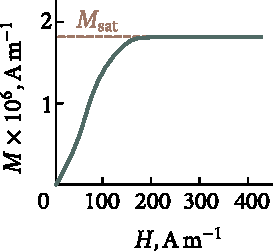
\includegraphics[scale=1]{figures/ch_07/fig_7_17.pdf}
			\caption[]{}
			\label{fig:7_17}
		\end{center}
	\end{minipage}
	\hfill{ }%space{-0.05cm}
	\begin{minipage}[t]{0.48\linewidth}
		\begin{center}
			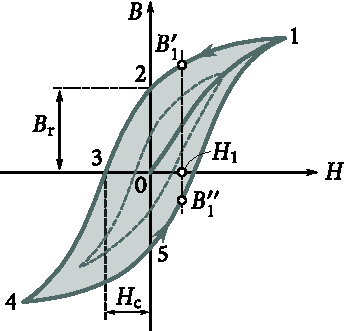
\includegraphics[scale=1]{figures/ch_07/fig_7_18.pdf}
			\caption[]{}
			\label{fig:7_18}
		\end{center}
	\end{minipage}
\vspace{-0.4cm}
\end{figure}

A magnetization curve for iron was first obtained and investigated in detail by the Russian scientist Aleksandr Stoletov (1839-1896).
The ballistic method of measuring the magnetic induction which he developed has been finding wide application (see \sect{8_3}).

Apart from the non-linear relation between $H$ and $M$ (or between $H$ and $B$), ferromagnetics are characterized by the presence of hysteresis.
If we bring magnetization up to saturation (point $1$ in \fig{7_18}) and then diminish the magnetic field strength, the induction $B$ will no longer follow the initial curve $0$-$1$, but will change in accordance with curve $1$-$2$.
As a result, when the strength of the external field vanishes (point $2$), the magnetization does not vanish and is characterized by the quantity $\ab{B}{r}$ called the \textbf{residual induction}.
The magnetization for this point has the value $\ab{M}{r}$ called the \textbf{retentivity} or \textbf{remanence}.

The magnetization vanishes only under the action of the field $\ab{H}{c}$ directed oppositely to the field that produced the magnetization.
The field strength $\ab{H}{c}$ is called the coercive force.

The existence of remanence makes it possible to manufacture permanent magnets, \ie, bodies that have a magnetic moment and produce a magnetic field in the space surrounding them without the expenditure of energy for maintaining the macroscopic currents.
A permanent magnet retains its properties better when the coercive force of the material it is made of is higher.

When an alternating magnetic field acts on a ferromagnetic, the induction changes in accordance with curve $1$-$2$-$3$-$4$-$5$-$1$ (\fig{7_18}) called a \textbf{hysteresis loop} (a similar curve is obtained in an $M$-$H$ diagram).
If the maximum values of $H$ are such that the magnetization reaches saturation, we get the so-called \textbf{maximum hysteresis loop} (the solid loop in \fig{7_18}).
If saturation is not reached at the amplitude values of $H$, we get a loop called a \textbf{partial cycle} (the dash line in the figure).
The number of such partial cycles is infinite, and all of them are within the maximum hysteresis loop.

Hysteresis results in the fact that the magnetization of a ferromagnetic is not a unique function of $H$.
It depends very greatly on the previous history of a specimen---on the fields which it was in previously.
For example, in a field of strength $H_1$ (\fig{7_18}), the induction may have any value ranging from $B_1'$ to $B_1''$.

It follows from everything said above about ferromagnetics that they are very similar in their properties to ferroelectrics (see \sect{2_9}).
In connection with the ambiguity of the dependence of $B$ on $H$, the concept of permeability is applied only to the initial magnetization curve.
The permeability of ferromagnetics $\mu$ (and, consequently, their magnetic susceptibility $\ab{\chi}{m}$) is a function of the field strength.
Figure \ref{fig:7_19}a shows an initial magnetization curve.
Let us draw from the origin of coordinates a siraight line that passes through an arbitrary point on the curve.
The slope of this line is proportional to the ratio $B/H$, \ie, to the permeability $\mu$ for the relevant value of the field strength.
When $H$ grows from zero, the slope (and, consequently, $\mu$) first grows. At point $2$ it reaches a maximum (straight line $0$-$2$ is a tangent to the curve) and then diminishes.
Figure \fig{7_19}b shows how $\mu$ depends on $H$.
A glance at the figure shows that the maximum value of the permeability is reached somewhat earlier than saturation.
Upon an unlimited increase in $H$, the permeability
approaches unity asymptotically.
This can be seen from the circumstance that $M$ in the expression $\mu=1+M/H$ cannot exceed the value $\ab{M}{sat}$.

\begin{figure}[!htb]
	\begin{center}
		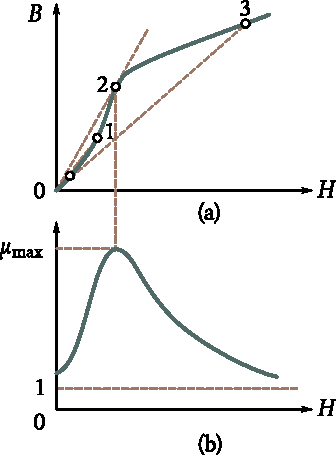
\includegraphics[scale=1]{figures/ch_07/fig_7_19.pdf}
		\caption[]{}
		\label{fig:7_19}
	\end{center}
	\vspace{-0.8cm}
\end{figure}

The quantities $\ab{B}{r}$ (or $\ab{M}{r}$), $\ab{H}{c}$ and $\ab{\mu}{max}$ are the basic characteristics of a ferromagnetic.
If the coercive force $\ab{H}{c}$ is great, the ferromagnetic is called \textbf{hard}.
It is characterized by a broad hysteresis loop.
A ferromagnetic with a low $\ab{H}{c}$ (and accordingly with a narrow hysteresis loop) is called \textbf{soft}.
The characteristic of a ferromagnetic is chosen depending on the use it is to be put to.
Thus, hard ferromagnetics are used for permanent magnets, and soft ones for the cores of transformers.
Table \ref{table:7_1} gives the characteristics of several typical ferromagnetics.

\begin{table}[!htb]
	\renewcommand{\arraystretch}{1.2}
	\caption{}
	\vspace{-0.6cm}
	\label{table:7_1}
	\begin{center}\resizebox{0.8\linewidth}{!}{
			\begin{tabular}{llccc}
				\toprule[1pt]
				\textbf{Substance} & \textbf{Composition} & $\ab{\mu}{max}$ & $\ab{B}{r}$, \si{\tesla} & $\ab{H}{c}$, \si{\ampere\per\metre}\\
				\midrule[0.5pt]\midrule[0.5pt]
				Iron & $99.9\%$ Fe & $5000$ & --- & $80$\\
                Supermalloy & $79\%$ Ni, $5\%$, Mo, $16\%$ Fe & $800000$ & --- & $0.3$\\
                Alniko & $10\%$ Al, $19\%$ Ni, $18\%$ Co & --- & $0.9$ & $52000$\\
				\bottomrule[1pt]
			\end{tabular}
	}\end{center}
\end{table}

The fundamentals of the theory of ferromagnetism were presented by the Soviet physicist Yakov Frenkel (1894-1952) and the German physicist Werner Heisenberg (1901-1976) in 1928.
It follows from experiments involving the studying of gyromagnetic phenomena (see \sect{7_6}) that the intrinsic (spin) magnetic moments of electrons are responsible for the magnetic properties of ferromagnetics.
In definite conditions, forces\footnote{These forces are called \textbf{exchange} ones. Their explanation is given only by quantum mehcanics.} may appear in crystals that make the magnetic moments of the electrons become lined up parallel to one another.
The result is the setting up of regions of \textbf{spontaneous magnetization}, also called \textbf{domains}.
Within the confines of each domain, a ferromagnetic is spontaneously magnetized to saturation and has a definite magnetic moment.
The directions of these moments are different for different domains (\fig{7_20}), so that in the absence of an external field the total moment of an entire body is zero.
Domains have dimensions of the order of \SIrange{1}{10}{\micro\metre}.

\begin{figure}[!htb]
	\begin{center}
		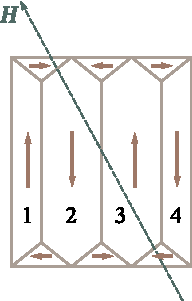
\includegraphics[scale=1]{figures/ch_07/fig_7_20.pdf}
		\caption[]{}
		\label{fig:7_20}
	\end{center}
	\vspace{-0.8cm}
\end{figure}

The action of a field on domains at different stages of the magnetization process is different.
First, with weak fields, displacement of the domain boundaries is observed.
As a result, the domains whose moments make a smaller angle with $\vec{H}$ grow at the expense of the domains for which the angle $\theta$ between the vectors $\ab{\vec{p}}{m}$ and $\vec{H}$ is greater.
For example, domains $1$ and $3$ in \fig{7_20} grow at the expense of domains $2$ and $4$.
With an increase in the field strength, this process goes on further and further until the domains with a smaller $\theta$ (which have a smaller energy in a magnetic field) completely absorb the domains that are less advantageous from the energy viewpoint.
In the next stage, the magnetic moments of the domains turn in the direction of the field.
The moments of the electrons within the confines of a domain turn simultaneously without violating their
strict parallelism to one another.
\textit{These processes (excluding slight displacements of the boundaries between the domains in very weak fields) are irreversible, and this is exactly what causes hysteresis}.

There is a definite temperature $\ab{T}{C}$ for every ferromagnetic at which the regions of spontaneous magnetization (domains) break up and the substance loses its ferromagnetic properties.
This temperature is called the \textbf{Curie point}. It is \SI{768}{\degreeCelsius} for iron and \SI{365}{\degreeCelsius} for nickel.
At a temperature above the Curie point, a ferromagnetic becomes an ordinary paramagnetic whose magnetic susceptibility obeys the \textbf{Curie-Weiss law}
\begin{equation}\label{eq:7_60}
    \ab{\chi}{m,mol} = \frac{C}{T - \ab{T}{C}}
\end{equation}

\noindent
[compare with \eqn{7_52}].
When a ferromagnetic is cooled to below its Curie point, domains once more appear in it.

Exchange forces sometimes result in the appearance of so-called \textbf{antiferromagnetics} (chromium, manganese, etc.).
The existence of antiferromagnetics was predicted by the Soviet physicist Lev Landau (1908-1968) in 1933.
In antiferromagnetics, the intrinsic magnetic moments of the electrons are spontaneously oriented antiparallel to one another.
Such an orientation involves adjacent atoms in
pairs.
The result is that antiferromagnetics have an extremely low magnetic susceptibility and behave like very weak paramagnetics.
There is also a temperature $\ab{T}{N}$ for antiferromagnetics at which the antiparallel orientation of the spins vanishes.
This temperature is known as the \textbf{antiferromagnetic Curie point} or the \textbf{Ne\'el point}.
Some antiferromagnetics (for example, erbium, dysprosium, alloys of manganese and copper) have two such points (an upper and a lower Neel point), the antiferromagnetic properties being observed only at the intermediate temperatures.
Above the upper point, the substance behaves like a paramagnetic, and at temperatures below the lower Ne\'el point it becomes a ferromagnetic.
